% Provenance (never printed): see sources/outline_sources.md (Year 2: taphonomy; index fossils;
% facies and fossils as environment markers; reconstructing a palaeoenvironment from a map and a
% section). Taphonomy after Loron (2024); live, dead and fossil assemblages after Tyler and
% Kowalewski (2025); Lagerstaetten after Gaines and others (2024), Mussini and Butterfield
% (2025), Vannier and others (2018), Gerschermann and others (2021) and Rauhut and others
% (2018); zone durations after Al-Suwaidi and others (2022); ichnofacies after Buatois and others
% (2020) and Paz and others (2023); stenohaline groups after McGairy and others (2021) and Saleh
% and others (2022). The Varden column from figdata/shared/region.py; porosities and rates from
% figdata/bachelor-2/palaeoenv.py; exercise and problem values in the Book 4 scratch calculator
% calc/ch20.py. The fossil content given to the Varden units is invented, like the region.
\chapter{Fossiles et paléoenvironnements}\label{ch:b2:palaeoenvironments}

Sur une dalle de grès gris, trois indices se détachent : la traînée qu'un trilobite a creusée dans la boue,
les rides qu'un courant a laissées derrière lui, et un terrier qu'un ver a creusé puis abandonné. Aucun de ces
indices n'est un animal entier, et pourtant ensemble ils disent que cette colline fut autrefois le fond d'une
mer, assez peu profonde pour que les vagues la remuent, assez salée pour que les trilobites y vivent. Les
fossiles sont les restes et les traces de la vie passée, et les géologues les lisent deux fois : comme des
horloges qui datent la roche, et comme des témoins du lieu où elle s'est formée. Ce chapitre suit un être vivant
depuis sa mort jusqu'au tiroir du collectionneur, ouvre les rares dépôts où même les parties molles se
conservent, puis lit l'environnement d'une mer disparue, avec des nombres, dans la couverture des Varden Hills.
% ledger: usgs:fossil-record-bulk, loron24:taphonomy

\begin{recall}
\textbf{Des volumes scolaires}~: fossile, moule, moulage et \omterm{def:b2:palaeoenvironments:fossil-kinds}{trace fossile}~; comment l'enfouissement et les
minéraux transforment une coquille en pierre~; la succession des fossiles au fil du temps.
\textbf{Du volume de première année}~: faciès sédimentaires et milieux de dépôt, turbidites, récifs et oolithes~; biozones,
fossiles stratigraphiques et datums de première apparition~; compaction, décompaction, loi d'Athy et épaisseur
solide d'une couche~; ciment~; accommodation. \textbf{Des chapitres précédents}~: transgressions et
régressions, le niveau marin à long terme et les \omterm{def:b2:phanerozoic-earth:oae}{événements anoxiques océaniques} (\cref{ch:b2:phanerozoic-earth}).
L'évolution des espèces et la classification des animaux et des plantes relèvent des volumes de biologie.
\end{recall}

\section{De la mort au fossile}\label{sec:b2:palaeoenvironments:taphonomy}

La plupart des êtres vivants ne laissent rien derrière eux. Bactéries et charognards consomment les
parties molles en quelques jours ou quelques années, les courants brisent et dispersent les parties dures,
et les acides des sols et des eaux interstitielles dissolvent ce qui reste. Un fossile est ce qui
résiste à tout cela, puis à l'enfouissement, au chauffage et au soulèvement de la roche qui le renferme.

\begin{definition}[Taphonomie~; potentiel de préservation]\label{def:b2:palaeoenvironments:taphonomy}
\emph{Taphonomie}\index{taphonomie} est l'étude de ce qui arrive aux
restes d'un organisme, de sa mort à sa découverte sous forme de fossile : décomposition,
charognage, transport, enfouissement, et changements chimiques de la diagenèse. Le
\emph{potentiel de préservation}\index{potentiel de préservation} d'un organisme, ou d'une
de ses parties, est la probabilité qu'il traverse ces étapes et survive dans la roche.
\end{definition}
% ledger: loron24:taphonomy

Chaque étape retire quelque chose, en ajoute, ou modifie quelque chose. La décomposition et le charognage
retirent les tissus mous~; des minéraux issus de l'eau interstitielle remplissent les pores d'un os ou
remplacent l'aragonite d'une coquille, ajoutant de la matière que l'animal n'avait jamais eue~; le chauffage
altère les molécules organiques qui subsistent. Loron classe toutes ces modifications post mortem en trois
types, gain, perte et altération, et les écrit comme une seule équation pour la variation de tout caractère
mesurable entre un organisme et son fossile. La figure ci-dessous suit les étapes et ce que chacune retire.
% ledger: loron24:taphonomy

\begin{omfigure}
\centering
\begin{tikzpicture}[font=\scriptsize, x=1cm, y=1cm,
  stage/.style={draw=black!60, fill=omSea!12, rounded corners=2pt, align=center,
    text width=2.05cm, minimum height=1.25cm, inner sep=2pt},
  loss/.style={align=center, text width=2.05cm, text=omThm!80!black}]
\node[stage] (a) at (0,0) {\textbf{mort}\\d'une\\communauté vivante};
\node[stage] (b) at (2.75,0) {\textbf{pourriture}\\\textbf{et charognage}\\sur le fond};
\node[stage] (c) at (5.5,0) {\textbf{transport}\\les courants trient\\et brisent};
\node[stage] (d) at (8.25,0) {\textbf{enfouissement}\\sous la couche\\active};
\node[stage] (e) at (11,0) {\textbf{diagenèse}\\compaction,\\remplacement};
\node[stage] (f) at (13.75,0) {\textbf{exhumation}\\et\\collecte};
\foreach \u/\v in {a/b, b/c, c/d, d/e, e/f} {\draw[-{Stealth[length=2mm]}, black!70] (\u) -- (\v);}
\node[loss, anchor=north] at (2.75,-0.8) {tissus mous perdus~;\\les squelettes se désagrègent};
\node[loss, anchor=north] at (5.5,-0.8) {parties légères emportées,\\coquilles brisées};
\node[loss, anchor=north] at (8.25,-0.8) {enfouissement lent~: davantage\\de temps pour les pertes};
\node[loss, anchor=north] at (11,-0.8) {aragonite dissoute,\\minéraux ajoutés};
\node[loss, anchor=north] at (13.75,-0.8) {érodés,\\ou jamais retrouvés};
\end{tikzpicture}
\par\smallskip{\small Le parcours taphonomique, d'une communauté vivante à une collection, avec
ce que chaque étape retire ou modifie. L'enfouissement est le tournant~: avant lui, les restes
sont exposés à toutes les pertes~; après lui, seules la diagenèse et l'érosion agissent sur eux.}
\end{omfigure}
% ledger: loron24:taphonomy

Les volumes scolaires appelaient fossile tout reste ou toute trace de vie passée conservée dans la
roche. Les deux types se comportent si différemment dans la roche qu'ils méritent leurs propres noms.

\begin{definition}[Fossile corporel~; trace fossile]\label{def:b2:palaeoenvironments:fossil-kinds} Un
\emph{fossile corporel}\index{fossile corporel} est une partie du corps d'un organisme, ou le moule ou le moulage
de cette partie : une coquille, un os, une dent, une feuille et, dans de rares dépôts, un tissu mou. Une
\emph{trace fossile}\index{trace fossile} est une structure qu'un organisme a produite par son activité dans ou
sur un sédiment ou une roche : une empreinte, une traînée, un terrier, un forage, un motif d'alimentation.
\end{definition}

Une \omterm{def:b2:palaeoenvironments:fossil-kinds}{trace fossile} fait partie du sédiment dans lequel elle a été creusée~: un courant qui la déplacerait
la détruirait. Elle enregistre donc les conditions du lieu même où vivait son auteur, ce qu'une coquille,
facilement roulée sur le fond, ne fait pas toujours. Les \omterm{def:b2:palaeoenvironments:fossil-kinds}{traces fossiles} se nomment comme des
organismes, avec un genre et une espèce, mais le nom décrit la structure, non l'animal~: un même terrier peut
être creusé par plusieurs sortes d'animaux, et un seul animal peut laisser plusieurs sortes de traces.

\subsection*{L'enfouissement contre la destruction}

La course entre l'enfouissement et la destruction peut se mettre dans un modèle simple.
Les restes posés sur le fond sont détruits à un taux constant $k$, la probabilité
par unité de temps qu'ils soient mangés, brisés ou dissous~; ils sont à l'abri dès
qu'une épaisseur $h$ de sédiment les recouvre, et le sédiment s'accumule au taux $s$.

\begin{proposition}[Enfouissement avant destruction]\label{prop:b2:palaeoenvironments:burial}
Sous ces hypothèses, la probabilité qu'un reste soit à l'abri est
\[
  P = e^{-kh/s}.
\]
Elle ne dépend des trois grandeurs qu'à travers le rapport du temps
d'enfouissement, $h/s$, à la durée moyenne de survie sur le fond, $1/k$.
\end{proposition}

\begin{proof}
Le reste doit attendre le temps $T = h/s$ pour être recouvert par l'épaisseur $h$. Avec un taux de
destruction $k$, la probabilité $p(t)$ de survivre jusqu'au temps $t$ obéit à $p' = -kp$, $p(0) =
1$, donc $p(t) = e^{-kt}$~; en $t = T$, cela vaut $e^{-kh/s}$.
\end{proof}

\begin{example}[Une coquille sur un fond calme]\label{ex:b2:palaeoenvironments:shell} Supposons
qu'une coquille survive en moyenne 20 ans sur le fond, $k = \qty{0.05}{an^{-1}}$, et soit à
l'abri sous $h = \qty{0.1}{m}$ de boue. À $s = \qty{1}{mm.an^{-1}}$, le temps d'enfouissement
est de 100 ans et $P = e^{-5} = 0.0067$~: moins d'une coquille sur cent survit. À \qty{1}{cm.an^{-1}},
$P = e^{-0.5} = 0.61$. Une tempête qui déverse \qty{0.3}{m} de sable en un jour enfouit
tout d'un coup, et alors $P$ est proche de un. Les nombres sont supposés, mais la leçon ne
l'est pas : les fossiles s'accumulent là où le sédiment arrive vite ou en couches soudaines.
\end{example}

Le modèle montre aussi pourquoi les archives sont biaisées. Un ver à corps mou, dont la durée moyenne de
survie sur le fond se compte en jours et non en décennies, a une valeur de $k$ des centaines de fois plus
grande qu'une coquille épaisse, et donc une chance exponentiellement plus faible. L'essentiel des archives
fossiles est fait d'animaux à coquille et de restes microscopiques. Tyler et Kowalewski ont mesuré combien
une communauté perd en chemin vers la roche. Sur 51 sites d'un fond marin côtier, ils ont compté 135
espèces vivantes d'invertébrés, 150 espèces parmi les coquilles et squelettes morts gisant sur le fond, et
112 qui ont aussi un enregistrement fossile. Les morts sont plus nombreux que les vivants parce que les
coquilles du fond se sont accumulées pendant de nombreuses années, issues d'animaux qui ne vivent plus là.
Les détritivores et les carnivores, surtout à corps mou, sont les moins susceptibles d'être conservés~;
pourtant les grands groupes écologiques de la communauté vivante ont tous été retrouvés parmi les morts.
% ledger: usgs:fossil-record-bulk, tyler25:live-dead, tyler25:soft-bodied

\section{Fenêtres de conservation exceptionnelle}\label{sec:b2:palaeoenvironments:lagerstatten}

\begin{definition}[Lagerstätte]\label{def:b2:palaeoenvironments:lagerstatte}
Une \emph{Lagerstätte}\index{Lagerstätte} (pluriel Lagerstätten) est un dépôt sédimentaire qui conserve
des fossiles d'une qualité exceptionnelle, en particulier les tissus mous, non biominéralisés, que la
décomposition détruit presque partout ailleurs~; un tel dépôt est aussi appelé Konservat-Lagerstätte.
\end{definition}
% ledger: gaines24:konservat

Les Lagerstätten sont rares, mais une grande part de ce que l'on sait des animaux à corps mou en
provient, et la première grande radiation des animaux, au Cambrien, se comprend le mieux à partir d'elles.
% ledger: gaines24:konservat

\subsection*{Le Burgess Shale}

En 1909, Charles Walcott dessina dans son carnet de terrain un petit arthropode qu'il avait trouvé dans
le Burgess Shale de Colombie-Britannique. Il en recueillit plus tard des centaines, \emph{Waptia}, dans
un seul intervalle d'environ \qty{2}{m} d'épaisseur, le Phyllopod Bed~; sa description moderne repose sur
plus de 1~800 spécimens conservés dans deux musées. Le Burgess Shale, vieux d'environ 508~Ma, s'est
déposé dans des eaux plus profondes, face à un escarpement sous-marin abrupt. Ses fossiles comprennent des
animaux sans coquille, conservés en films aplatis de carbone, souvent des corps entiers. Une telle
conservation est liée à un enfouissement dans des boues pauvres en oxygène, que les animaux ne fouissaient pas
et que les courants ne remaniaient pas~: les pertes de la figure ci-dessus étaient arrêtées d'un coup.
% ledger: vannier18:waptia, mussini25:burgess

\begin{omfigure}
\centering
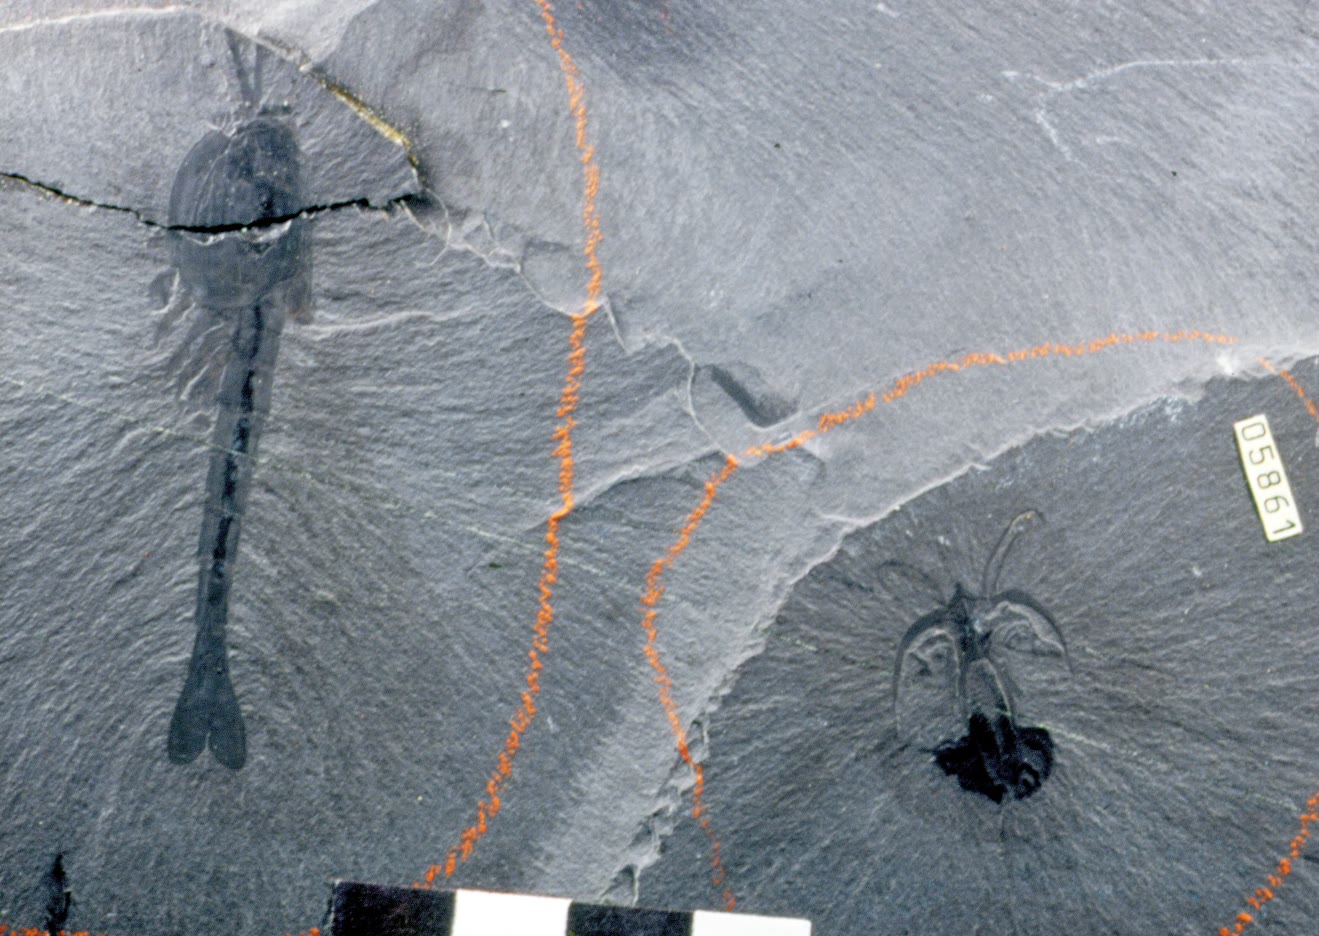
\includegraphics[width=0.72\linewidth]{images/book4/b2-20-burgess-waptia-marrella.jpg}
\par\smallskip{\small Deux arthropodes du Burgess Shale, conservés en
films sombres de carbone~: \emph{Waptia} (à gauche) et \emph{Marrella}
(à droite). (James St.~John, CC~BY~2.0, via Wikimedia Commons.)}
\end{omfigure}
% ledger: mussini25:burgess

\subsection*{Solnhofen}

Les calcaires à grain fin de Solnhofen et d'Eichstätt, en Bavière, se sont déposés dans des lagunes au
début du Tithonien, dernier âge du Jurassique, qui a commencé il y a \qty{149.2}{Ma}. Ils sont la localité
type de douze spécimens d'\emph{Archaeopteryx}, de nombreux ptérosaures et de poissons dont les tissus
mous et même les motifs de couleur subsistent. Les fossiles y sont rares, mais leur conservation est
exceptionnelle. Plusieurs conditions ont été proposées, agissant peut-être ensemble~: des eaux de fond environ
trois fois plus salées que l'eau de mer, ou très alcalines, qui ralentissent la décomposition
bactérienne~; des tapis de bactéries qui scellaient les carcasses~; des eaux de fond sans oxygène, qui tenaient
à distance les charognards~; et des tempêtes qui remuaient la boue calcaire et enfouissaient vite les
carcasses. Chacune d'elles allonge le temps de survie $1/k$ ou raccourcit le temps d'enfouissement $h/s$.
% ledger: gerschermann21:solnhofen, rauhut18:archaeopteryx, ics4:jurassic-stages

\begin{omfigure}
\centering
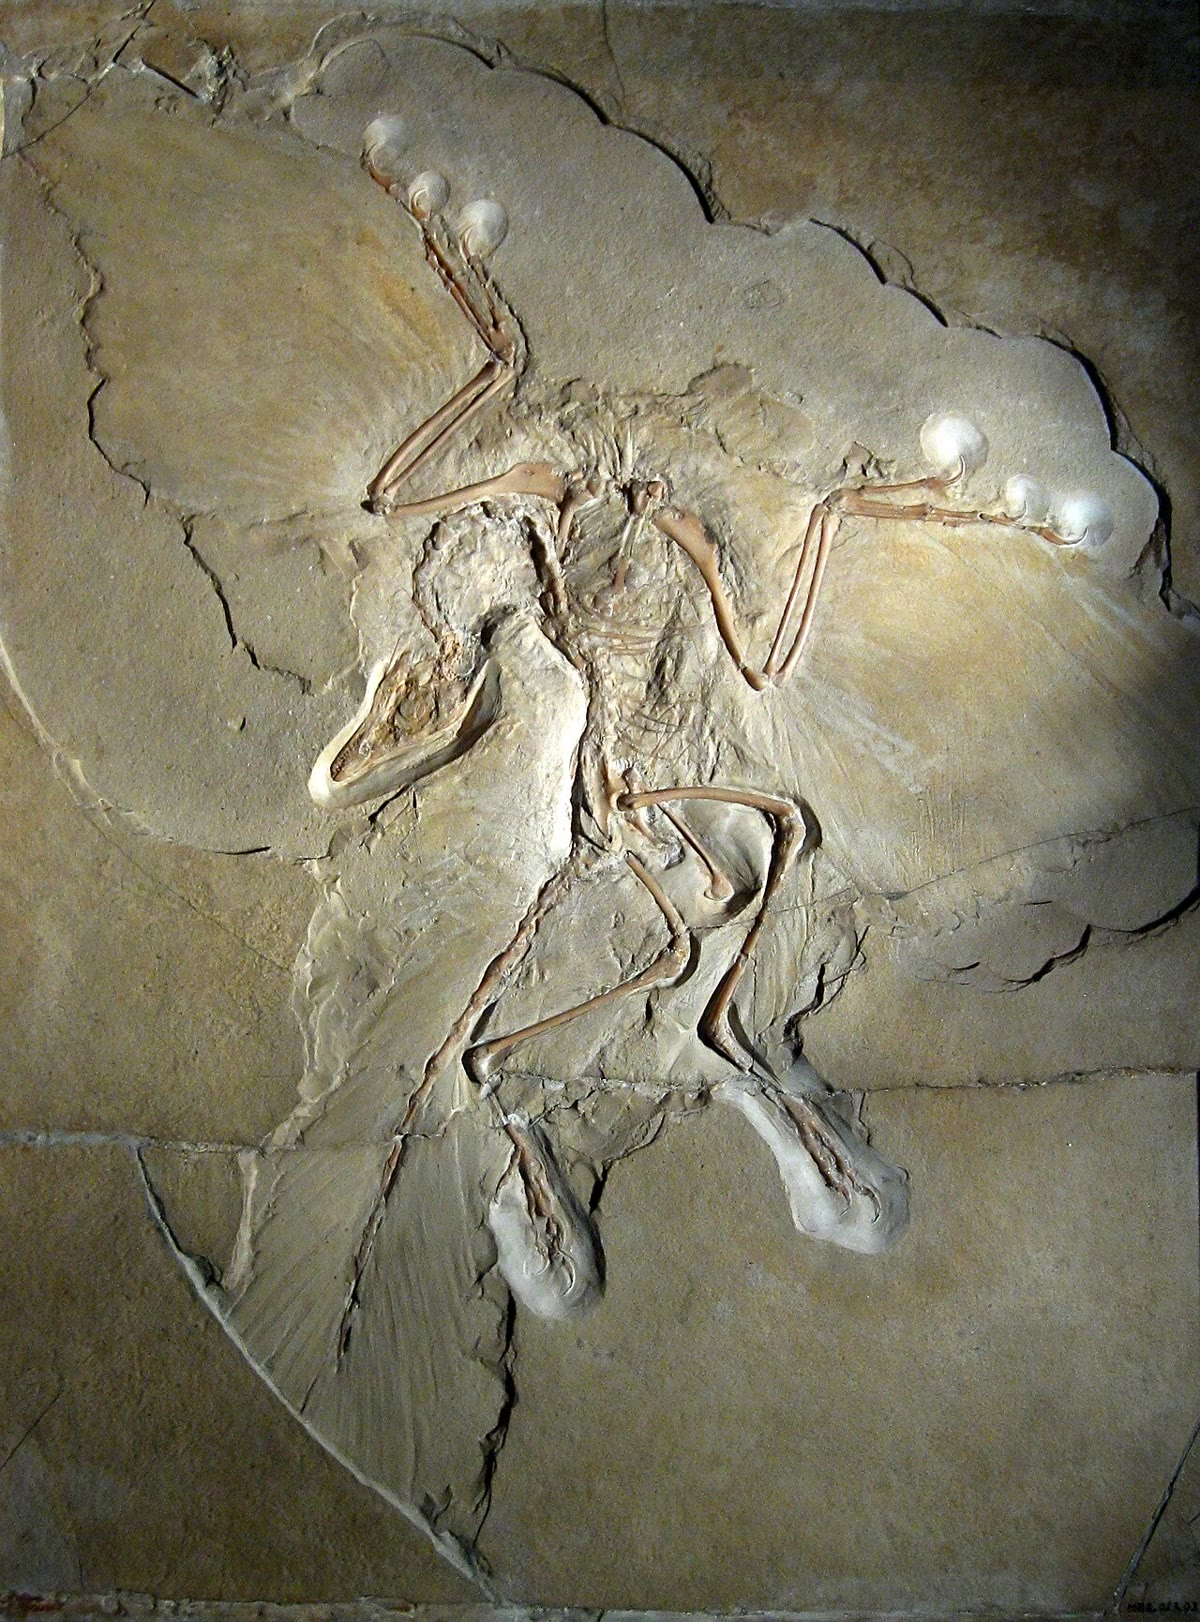
\includegraphics[width=0.5\linewidth]{images/book4/b2-20-archaeopteryx-berlin.jpg}
\par\smallskip{\small Le spécimen de Berlin d'\emph{Archaeopteryx}, issu
des calcaires de Solnhofen~: les os et les empreintes des plumes des
ailes et de la queue. (H.~Raab, CC~BY-SA~3.0, via Wikimedia Commons.)}
\end{omfigure}
% ledger: rauhut18:archaeopteryx, gerschermann21:solnhofen

\subsection*{Les fossiles comme horloges}

Le volume de première année a construit la biozone, un ensemble de couches défini par ses fossiles, et le fossile
stratigraphique qui la reconnaît. Quelle horloge fine forment-ils~? Une zone à ammonites du Jurassique peut
durer environ un million d'années~: la plus ancienne zone toarcienne, datée par les âges uranium--plomb de
niveaux de cendres en Argentine, s'étend de 183.73 à \qty{182.77}{Ma}. Les zones se divisent en horizons, et au
Jurassique supérieur un horizon à ammonites dure en moyenne \qty{165}{ka}. Tous les squelettes d'\emph{Archaeopteryx}
proviennent d'une seule zone qui compte cinq horizons, si bien que l'oiseau est connu sur quelque 0.7
à 1~Ma. Les fossiles ne donnent toutefois qu'un ordre~; les âges en années viennent de niveaux de cendres datés
à l'uranium et au plomb, et de cycles sédimentaires. Les mêmes niveaux placent la base du Toarcien à $183.73$,
avec une incertitude de $+0.35$ et \qty{-0.50}{Ma}, là où la charte internationale donne \qty{184.2}{Ma}.
% ledger: alsuwaidi22:toarcian, rauhut18:archaeopteryx, ics4:jurassic-stages

\section{Les fossiles comme témoins du milieu}\label{sec:b2:palaeoenvironments:environment}

Pour lire un milieu dans un fossile, le géologue suppose que l'organisme vivait là où vivent ses apparentés
actuels, et que les processus qui agissent aujourd'hui sur les sédiments agissaient de la même façon alors.

\begin{definition}[Actualisme]\label{def:b2:palaeoenvironments:actualism} \emph{Actualisme}\index{actualisme}
est la méthode qui interprète les archives géologiques passées par les processus,
et par les relations entre organismes et leur milieu, qui peuvent être observés aujourd'hui.
\end{definition}

En 1830, Charles Lyell donna au premier tome de ses \emph{Principles of Geology} (Principes
de géologie) le sous-titre « une tentative d'expliquer les anciens changements de la surface
de la Terre, par référence à des causes encore à l'œuvre ». La méthode a des limites. De
nombreux groupes sont éteints, et leur mode de vie doit être déduit de leur forme et des sédiments
qui les entourent~; et un milieu du passé peut n'avoir aucun équivalent exact aujourd'hui.
% ledger: lyell1830:title

\begin{definition}[Paléoenvironnement]\label{def:b2:palaeoenvironments:palaeoenvironment}
Un \emph{paléoenvironnement}\index{paléoenvironnement} est l'ensemble
des conditions physiques, chimiques et biologiques qui régnaient là où et quand
une roche s'est formée~: le cadre, la profondeur et l'énergie de l'eau, sa
salinité, sa température et son oxygène, la nature du fond et la vie qui s'y trouve.
\end{definition}

\subsection*{Où vivait le fossile~?}

La première question est de savoir si les fossiles ont vécu là où ils gisent.

\begin{definition}[Biocénoses et thanatocénoses~; fossiles autochtones et
allochtones]\label{def:b2:palaeoenvironments:assemblages} Une \emph{biocénose}\index{biocénose} est un ensemble
de fossiles d'organismes qui ont vécu ensemble, conservés là où et comme ils ont vécu~;
une \emph{thanatocénose}\index{thanatocénose} est un ensemble de restes rassemblés après la
mort, qui peut mêler des organismes de lieux et d'époques différents. Un fossile est
\emph{autochtone}\index{fossile autochtone} s'il est conservé là où vivait l'organisme, et
\emph{allochtone}\index{fossile allochtone} s'il a été transporté d'ailleurs avant son enfouissement.
\end{definition}

Les indices sont ceux du transport. Des coquilles encore fermées, un corail ou un bivalve fouisseur dans sa
position de croissance, des épines fragiles intactes, toutes les classes d'âge d'une population présentes~:
les fossiles sont vraisemblablement \omterm{def:b2:alpine-orogen:nappes}{autochtones}. Des valves isolées triées par taille, des fragments usés et
brisés, des coquilles concentrées à la base d'un lit granoclassé~: elles ont été transportées. Une \omterm{def:b2:palaeoenvironments:assemblages}{thanatocénose}
de coquilles, comme celle du fond côtier décrit plus haut, conserve encore l'essentiel de la communauté,
mais elle rassemble de nombreuses années en une seule couche~: ses fossiles sont moyennés dans le temps.
% ledger: tyler25:live-dead

\subsection*{Salinité et oxygène}

Certains animaux ne tolèrent que la salinité de la pleine mer~: on les dit sténohalins. Échinodermes,
céphalopodes, coraux et, au Paléozoïque, trilobites sont des groupes sténohalins typiques~; leur présence témoigne
d'une eau de mer normale, et leur absence d'une faune riche peut témoigner contre elle. Les dépôts d'un estuaire
silurien au Viêt Nam renferment des débris végétaux, des arêtes de poissons, des bivalves, des gastéropodes
et des ostracodes, mais aucun de ces groupes. Les échinodermes manquent aussi dans la biote de Chengjiang,
une \omterm{def:b2:palaeoenvironments:lagerstatte}{Lagerstätte} vieille d'environ 518~Ma, bien qu'ils se trouvent dans des Lagerstätten marines ouvertes du
Cambrien~: les animaux de Chengjiang vivaient près d'un delta, où l'eau douce faisait fluctuer la salinité.
% ledger: mcgairy21:stenohaline, saleh22:echinoderms, saleh22:age

L'oxygène laisse sa marque par l'intermédiaire des fouisseurs. Là où l'eau de fond contient
de l'oxygène, les animaux mélangent le sédiment et détruisent sa lamination fine~; là où
il n'y en a pas, les laminations se conservent, les terriers sont absents et la pyrite se
forme, comme dans les schistes noirs des \omterm{def:b2:phanerozoic-earth:oae}{événements anoxiques océaniques} du
\cref{ch:b2:phanerozoic-earth}. Ce même manque de fouisseurs a protégé les carcasses du Burgess Shale.
% ledger: mussini25:burgess

\subsection*{Ichnofaciès}

Les \omterm{def:b2:palaeoenvironments:fossil-kinds}{traces fossiles} sont les meilleurs témoins du fond, puisqu'elles n'ont pas été déplacées.
Leurs auteurs réagissent à l'énergie de l'eau, à la fermeté du fond, à la nourriture
et à l'oxygène, et les mêmes associations de traces reviennent au fil du Phanérozoïque.

\begin{definition}[Ichnofaciès]\label{def:b2:palaeoenvironments:ichnofacies} Un
\emph{ichnofaciès}\index{ichnofaciès} est une association récurrente de \omterm{def:b2:palaeoenvironments:fossil-kinds}{traces fossiles} qui
traduit un ensemble de conditions du milieu~; il porte le nom d'une trace caractéristique.
\end{definition}

Le long d'un profil marin, du rivage au bassin profond, quatre \omterm{def:b2:palaeoenvironments:ichnofacies}{ichnofaciès} marins se succèdent l'un
après l'autre (figure ci-dessous). L'\omterm{def:b2:palaeoenvironments:ichnofacies}{ichnofaciès} à \emph{Skolithos}, dominé par des terriers verticaux,
cylindriques ou en U d'animaux suspensivores, avec peu de traces horizontales, est typique de l'estran
et de l'avant-côte. L'\omterm{def:b2:palaeoenvironments:ichnofacies}{ichnofaciès} à \emph{Cruziana}, dominé par les terriers de déposivores, avec les
traces de brouteurs, de carnivores et de suspensivores, est typique du large~: le fond situé entre la
base de la vague de beau temps, profondeur au-dessus de laquelle les vagues ordinaires remuent le sédiment,
et la base de la vague de tempête, atteinte seulement par les tempêtes. L'\omterm{def:b2:palaeoenvironments:ichnofacies}{ichnofaciès} à \emph{Zoophycos},
nommé d'après un terrier qui remanie le sédiment en feuillets hélicoïdaux autour d'un axe central,
est typique du plateau au-dessous de la base de la vague de tempête et du talus. L'\omterm{def:b2:palaeoenvironments:ichnofacies}{ichnofaciès} à
\emph{Nereites}, aux méandres, spirales et réseaux réguliers, lus comme les pièges et les jardins d'animaux
qui trouvent peu de nourriture, est typique de la mer profonde au-delà de la rupture de pente. Dans
les baies saumâtres et les estuaires, un \omterm{def:b2:palaeoenvironments:ichnofacies}{ichnofaciès} à Cruziana d'espèces peu nombreuses est la règle.
% ledger: buatois20:ichnofacies, miguez21:ichnofacies, zhang15:zoophycos, buatois25:graphoglyptids, paz23:nereites

\begin{omfigure}
\centering
\begin{tikzpicture}[font=\scriptsize, x=1cm, y=1cm]
% sea and floor (schematic, not to scale)
\fill[omSea!20] (0.6,0) -- (14,0) -- (14,-3.6) -- (11.2,-3.6) -- (9.6,-1.9) -- (6.2,-1.5)
  -- (3.2,-0.9) -- (1.2,-0.15) -- cycle;
\fill[omLithSand!45] (0,0.25) -- (0.6,0) -- (1.2,-0.15) -- (3.2,-0.9) -- (6.2,-1.5)
  -- (9.6,-1.9) -- (11.2,-3.6) -- (14,-3.6) -- (14,-4.3) -- (0,-4.3) -- cycle;
\draw[black!70, line width=0.6pt] (0,0.25) -- (0.6,0) -- (1.2,-0.15) -- (3.2,-0.9) -- (6.2,-1.5)
  -- (9.6,-1.9) -- (11.2,-3.6) -- (14,-3.6);
\draw[omSea!80!black, line width=0.6pt] (0.6,0) -- (14,0);
\node[anchor=south east, omSea!80!black] at (14,0) {niveau de la mer};
% wave bases
\draw[dashed, black!60] (2.133,-0.5) -- (14,-0.5) node[anchor=south east, black!70] {base de la vague de beau temps};
\draw[dashed, black!60] (4.7,-1.2) -- (14,-1.2) node[anchor=south east, black!70] {base de la vague de tempête};
% zone labels
\node[align=center] at (1.9,0.55) {estran,\\avant-côte};
\node[align=center] at (4.6,0.55) {large};
\node[align=center] at (8.0,0.55) {plateau};
\node[align=center] at (10.5,0.55) {talus};
\node[align=center] at (12.7,0.55) {bassin};
% Skolithos: vertical tubes
\foreach \x in {1.75,1.95,2.15,2.35} {\draw[black!80, line width=0.7pt] (\x,{-0.15-0.375*(\x-1.2)}) -- ++(0,-0.55);}
\node[align=center] at (2.1,-2.15) {\textbf{\emph{Skolithos}}\\tubes verticaux};
% Cruziana: horizontal bilobed trails
\foreach \x in {4.0,4.8} {\draw[black!80, line width=0.6pt] (\x,-1.45) .. controls ++(0.2,0.08) .. ++(0.5,0);
  \draw[black!80, line width=0.6pt] (\x,-1.53) .. controls ++(0.2,-0.08) .. ++(0.5,0);}
\node[align=center] at (4.7,-2.35) {\textbf{\emph{Cruziana}}\\terriers de nourrissage,\\traces de broutage};
% Zoophycos: spreite arcs
\foreach \r in {0.12,0.22,0.32} {\draw[black!80, line width=0.5pt] (8.0,-2.25) ++(-\r,0) arc (180:360:\r cm and 0.5*\r cm);}
\draw[black!80, line width=0.6pt] (8.0,-2.25) -- (8.0,-1.8);
\node[align=center] at (8.0,-3.05) {\textbf{\emph{Zoophycos}}\\feuillets\\hélicoïdaux};
% Nereites: meander
\draw[black!80, line width=0.6pt, domain=0:2.2, samples=80, smooth] plot (12.0+\x*0.5,{-3.9+0.12*sin(\x*720)});
\node[align=center, anchor=north] at (12.5,-4.35) {\textbf{\emph{Nereites}}\\méandres, réseaux};
\end{tikzpicture}
\par\smallskip{\small Les quatre \omterm{def:b2:palaeoenvironments:ichnofacies}{ichnofaciès} marins du modèle de Seilacher, le long d'un profil du rivage au
bassin profond, avec un croquis d'une trace caractéristique de chacun~; les profondeurs ne sont pas à l'échelle.
Les traces répondent davantage à l'énergie, à la nourriture et à l'oxygène qu'à la profondeur en elle-même.}
\end{omfigure}
% ledger: buatois20:ichnofacies, miguez21:ichnofacies, zhang15:zoophycos, buatois25:graphoglyptids, paz23:nereites

La profondeur n'agit pas directement. Dans un chenal de mer profonde, où les courants de turbidité
sont forts, des terriers verticaux de l'\omterm{def:b2:palaeoenvironments:ichnofacies}{ichnofaciès} à Skolithos apparaissent loin sous toute
base de vague~; et près d'un delta, où l'eau douce et la boue se déversent, les traces du
large sont plus pauvres qu'ailleurs. Les auteurs ont aussi changé au fil du temps~: le terrier
\emph{Zoophycos} vivait sur le plateau au Paléozoïque, sur le plateau inférieur et le talus au
Mésozoïque, et en mer profonde au Cénozoïque. Un \omterm{def:b2:palaeoenvironments:ichnofacies}{ichnofaciès} enregistre les conditions du fond,
dont la profondeur n'est qu'inférée, et cette inférence doit tenir compte de l'âge de la roche.
% ledger: buatois20:ichnofacies, zhang15:zoophycos

\begin{inthefield}[Compter les fossiles couche par couche]
Un paléontologue qui reconstruit un milieu à partir d'une coupe consigne chaque lit avec sa lithologie,
son épaisseur et ses structures sédimentaires, puis ses fossiles : quels groupes, combien, si les
coquilles sont entières ou brisées, fermées ou ouvertes, triées ou non, et dans quelle position elles
gisent. Les \omterm{def:b2:palaeoenvironments:fossil-kinds}{traces fossiles} sont notées là où on les voit, sur les surfaces de stratification et
dans les faces verticales, avec la profondeur à laquelle atteignent les terriers. Comme une coquille
peut être déplacée mais un terrier non, les deux listes sont tenues séparées~: le milieu se lit d'abord
dans les traces, puis les \omterm{def:b2:palaeoenvironments:fossil-kinds}{fossiles corporels} sont contrôlés pour détecter les signes de transport.
\end{inthefield}

\begin{omfigure}
\centering
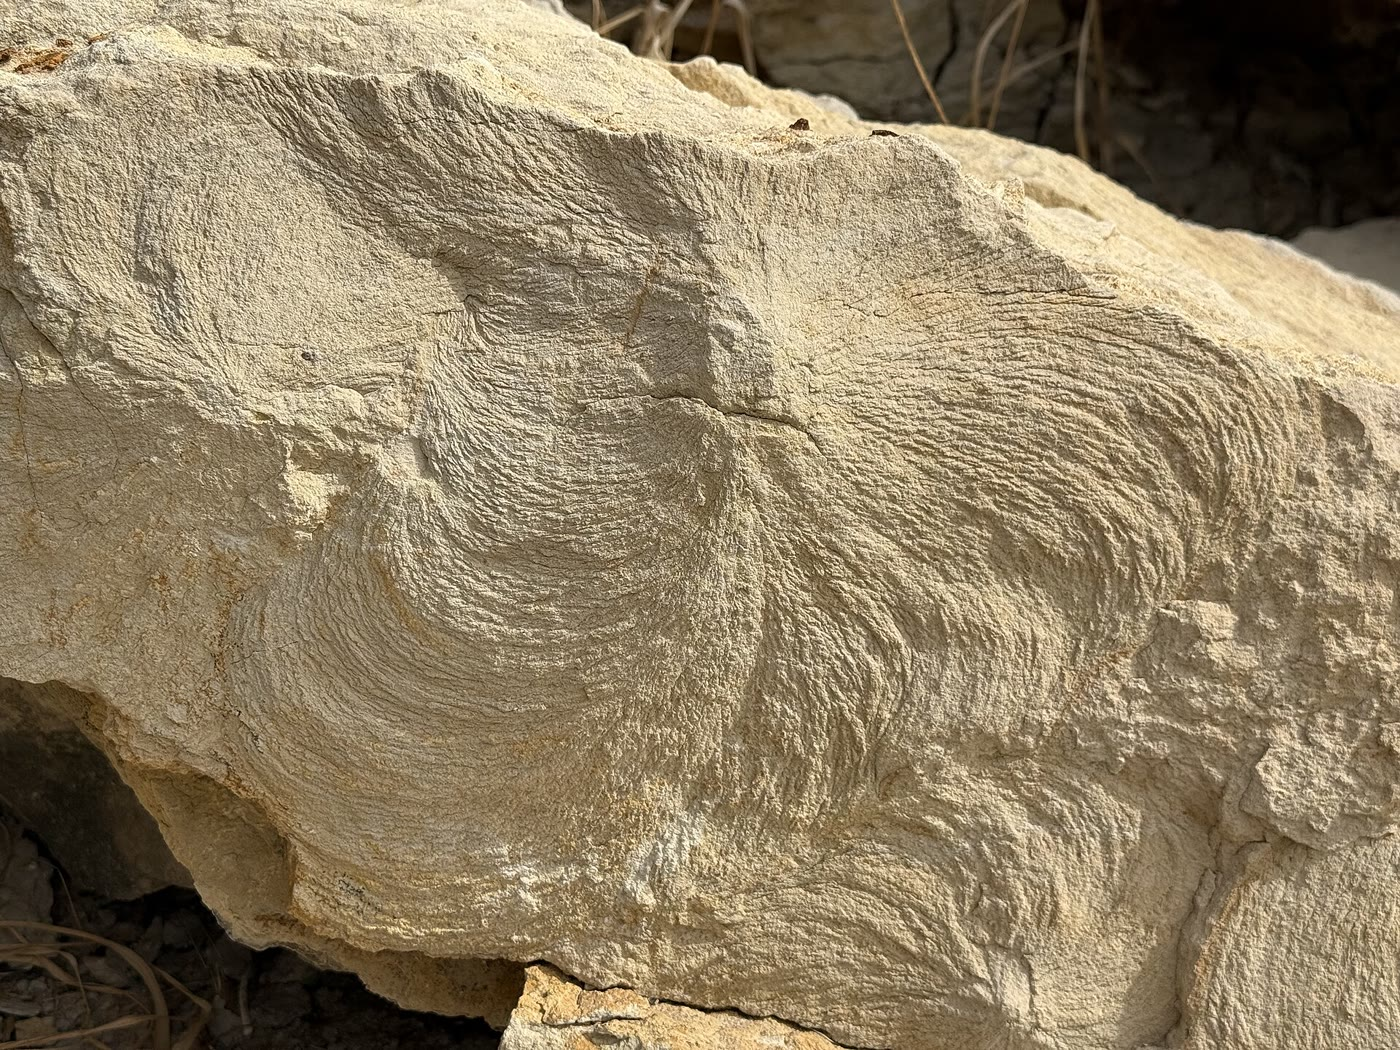
\includegraphics[width=0.5\linewidth]{images/book4/b2-20-zoophycos.jpg}
\par\smallskip{\small \emph{Zoophycos} dans un bloc à Sagres, au Portugal~: les arcs sont les
lamelles d'une \omterm{def:b2:alpine-orogen:nappes}{nappe} hélicoïdale de sédiment remanié. (Amada44, CC~BY~4.0, via Wikimedia Commons.)}
\end{omfigure}
% ledger: zhang15:zoophycos

\section{Lire une mer disparue}\label{sec:b2:palaeoenvironments:varden}

Les milieux se succèdent côte à côte~: une plage, un fond au large, un plateau plus profond.
Lorsque la mer monte ou que le fond s'enfonce, chaque milieu se déplace vers la terre
au-dessus de son voisin, et ses dépôts viennent se placer sur ceux du voisin. Une succession
verticale de faciès, sans coupure, répète donc l'ordre des milieux qui se trouvaient
côte à côte~; le volume de troisième année fait de cette règle, la loi de Walther, son point
de départ. Une coupe lue de bas en haut est un film du rivage qui traverse un même lieu.

La couverture des Varden Hills, la région inventée de la série, en fournit un exemple
complet. Ses épaisseurs sont celles du modèle de la région~; les fossiles de la figure
ci-dessous sont inventés pour elle, mais chacun est choisi parmi ceux que des roches de
ce type peuvent contenir. Le calcaire reçoit le Toarcien, de 184.2 à \qty{174.7}{Ma},
et l'argilite l'Aalénien au Callovien, de \qty{174.7}{Ma} à \qty{161.5}{Ma}.
% ledger: data:b4-palaeoenv, ics4:jurassic-stages

\begin{omfigure}
\centering
% figdata/bachelor-2/palaeoenv.py part log (thicknesses from figdata/shared/region.py)
\begin{tikzpicture}[x=1cm, y=0.0165cm, font=\scriptsize]
% scale
\draw[black!70] (-0.35,0) -- (-0.35,460);
\foreach \z in {0,100,...,400} {\draw[black!70] (-0.45,\z) -- (-0.35,\z) node[left=3pt] {\z};}
\node[rotate=90, anchor=south] at (-1.15,230) {hauteur au-dessus de la base de la couverture (m)};
% units
\fill[lith sandstone] (0,0) rectangle (2.2,120);
\fill[lith limestone] (0,120) rectangle (2.0,180);
\fill[lith limestone] (0,180) rectangle (1.6,300);
\fill[lith shale] (0,300) rectangle (1.1,400);
\fill[om lith={icsCretaceous!35}{om limestone}] (0,400) -- (1.4,400) -- (1.4,452)
  .. controls (1.0,466) and (0.6,446) .. (0.3,458) -- (0,455) -- cycle;
\draw[black!70] (0,0) rectangle (2.2,120);
\draw[black!70] (0,120) rectangle (2.0,180);
\draw[black!70] (0,180) rectangle (1.6,300);
\draw[black!70] (0,300) rectangle (1.1,400);
\draw[black!70] (0,400) -- (1.4,400) -- (1.4,452) .. controls (1.0,466) and (0.6,446) ..
  (0.3,458) -- (0,455) -- cycle;
\node[anchor=west, font=\tiny] at (1.45,460) {sommet érodé};
% unit names
\node[anchor=west, align=left] at (2.6,60) {\textbf{grès}, \qty{120}{m}\\Trias};
\node[anchor=west, align=left] at (2.6,150) {\textbf{calcaire oolithique}, \qty{60}{m}\\Toarcien};
\node[anchor=west, align=left] at (2.6,240) {\textbf{calcaire fin}, \qty{120}{m}\\Toarcien};
\node[anchor=west, align=left] at (2.6,350) {\textbf{argilite}, \qty{100}{m}\\Aalénien--Callovien};
\node[anchor=west, align=left] at (2.6,424) {\textbf{craie}\\Crétacé};
% content
\node[anchor=west, align=left, text width=6.9cm] at (6.3,60) {stratifications obliques de chenaux sur des
  bases érodées; traces de racines; fragments de plantes; aucun fossile marin};
\node[anchor=west, align=left, text width=6.9cm] at (6.3,150) {oolithes à stratification oblique; tubes verticaux
  et terriers en U; fragments de coquilles usés};
\node[anchor=west, align=left, text width=6.9cm] at (6.3,240) {ossicules de crinoïdes, brachiopodes,
  bélemnites, ammonites; traînées de reptation et terriers de nourrissage; lits de coquilles brisées à base
  nette};
\node[anchor=west, align=left, text width=6.9cm] at (6.3,350) {gris sombre, localement laminé;
  pyrite; ammonites et bivalves à coquille mince; terriers hélicoïdaux à feuillets dans les lits plus clairs};
\node[anchor=west, align=left, text width=6.9cm] at (6.3,424) {coccolithes; échinides, éponges;
  nodules de silex; bioturbée partout};
\foreach \z in {120,180,300,400} {\draw[black!25] (2.25,\z) -- (13.2,\z);}
\node[font=\scriptsize\bfseries, anchor=south west] at (2.6,462) {unité et âge};
\node[font=\scriptsize\bfseries, anchor=south west] at (6.3,462) {contenu des lits};
\end{tikzpicture}
\par\smallskip{\small La couverture des Varden Hills sous forme de coupe, avec le contenu de ses unités.
Les épaisseurs sont celles du modèle de la région, sauf la craie, dont le sommet érodé est ici tronqué
(\qty{766}{m} d'épaisseur dans le synclinal, \cref{ex:b2:palaeoenvironments:shale})~; la largeur de
la colonne croît avec la taille du grain~; les fossiles et leurs âges sont inventés pour la région.}
\end{omfigure}
% ledger: data:b4-palaeoenv, ics4:jurassic-stages

\begin{example}[La base de la couverture de Varden]\label{ex:b2:palaeoenvironments:base}
Le grès renferme des remplissages de chenaux à bases érodées, des racines et des fragments de plantes, et aucun
fossile marin~: il a été déposé par des rivières sur la terre ferme. Le calcaire oolithique au-dessus présente
des oolithes à stratification oblique, qui grossissent en roulant dans une eau agitée, des tubes verticaux et des
terriers en U de l'\omterm{def:b2:palaeoenvironments:ichnofacies}{ichnofaciès} à Skolithos, et des fragments de coquilles usés, tous \omterm{def:b2:alpine-orogen:nappes}{allochtones}~: un haut-fond
de l'avant-côte, balayé par les vagues. Entre les deux, la mer est arrivée~: le contact enregistre une \omterm{def:b2:phanerozoic-earth:transgression}{transgression
marine}. Dans l'ordre de la loi de Walther, la plaine fluviale a été suivie du rivage, puis du haut-fond.
\end{example}
% ledger: buatois20:ichnofacies

\subsection*{À quelle vitesse le fond marin s'est-il comblé~?}

Une biozone donne une durée, une coupe donne une épaisseur, et leur
rapport est un taux. Mais l'épaisseur a diminué depuis le dépôt du sédiment~:
l'eau des pores a été chassée, et les grains seuls se conservent.

\begin{proposition}[Taux d'accumulation d'une couche compactée]\label{prop:b2:palaeoenvironments:rate}
Une couche d'épaisseur actuelle $h$ et de porosité moyenne $\varphi$, déposée
pendant le temps $\Delta t$ avec la porosité $\varphi_0$, s'est accumulée au taux
\[
  r = \frac{h\,(1 - \varphi)}{(1 - \varphi_0)\,\Delta t}
\]
de sédiment frais, et au taux $h(1-\varphi)/\Delta t$
de grains, qui ne dépend pas de $\varphi_0$.
\end{proposition}

\begin{proof}
Par unité de surface, la couche contient le volume de grains $h(1 - \varphi)$, l'épaisseur solide du
volume de première année. La compaction chasse l'eau sans ajouter ni retirer de grains, si bien que le
sédiment frais, de porosité $\varphi_0$, avait l'épaisseur $h_0$ avec $h_0(1 - \varphi_0) = h(1 -
\varphi)$. En divisant $h_0$ et l'épaisseur solide par $\Delta t$, on obtient les deux taux.
\end{proof}

Lorsque la porosité n'a pas été mesurée, la loi d'Athy la donne en fonction de la profondeur. La figure
ci-dessous montre la loi pour quatre lithologies, et le facteur $(1 - \varphi(z))/(1 - \varphi_0)$ par lequel
une couche mince située à la profondeur $z$ doit être étirée pour retrouver son épaisseur en surface. La
craie et l'argilite commencent avec beaucoup d'eau et la perdent vite~: une couche mince
d'argilite à \qty{1000}{m} était 1.68 fois plus épaisse lors de son dépôt, une couche de craie 2.19 fois.
% ledger: pybacktrack:compaction, pybacktrack4:limestone, data:b4-palaeoenv

\begin{omfigure}
\centering
% figdata/bachelor-2/palaeoenv.py parts poro and ratio
\begin{tikzpicture}
\begin{groupplot}[group style={group size=2 by 1, horizontal sep=1.6cm},
  width=0.46\linewidth, height=6.2cm, y dir=reverse, ymin=0, ymax=3000,
  tick label style={font=\scriptsize}, label style={font=\small}, xtick pos=bottom,
  ytick pos=left, scaled y ticks=false, yticklabel style={/pgf/number format/1000 sep={\,}}]
\nextgroupplot[xmin=0, xmax=0.75, xlabel={porosité $\varphi$}, ylabel={profondeur $z$ (\unit{m})},
  legend style={at={(0.5,1.04)}, anchor=south, draw=none, font=\scriptsize, legend columns=2}]
\addplot[omThm, line width=1pt] table[x=shale, y=z_m] {figdata/out/bachelor-2-palaeoenv-poro.dat};
\addlegendentry{argilite}
\addplot[omSea!80!black, line width=1pt, dashed] table[x=sandstone, y=z_m] {figdata/out/bachelor-2-palaeoenv-poro.dat};
\addlegendentry{grès}
\addplot[black, line width=1pt, dotted] table[x=chalk, y=z_m] {figdata/out/bachelor-2-palaeoenv-poro.dat};
\addlegendentry{craie}
\addplot[green!45!black, line width=1pt, dash dot] table[x=limestone, y=z_m] {figdata/out/bachelor-2-palaeoenv-poro.dat};
\addlegendentry{calcaire}
\nextgroupplot[xmin=1, xmax=3.2, xlabel={facteur de restauration $(1-\varphi)/(1-\varphi_0)$}]
\addplot[omThm, line width=1pt] table[x=shale, y=z_m] {figdata/out/bachelor-2-palaeoenv-ratio.dat};
\addplot[omSea!80!black, line width=1pt, dashed] table[x=sandstone, y=z_m] {figdata/out/bachelor-2-palaeoenv-ratio.dat};
\addplot[black, line width=1pt, dotted] table[x=chalk, y=z_m] {figdata/out/bachelor-2-palaeoenv-ratio.dat};
\addplot[green!45!black, line width=1pt, dash dot] table[x=limestone, y=z_m] {figdata/out/bachelor-2-palaeoenv-ratio.dat};
\end{groupplot}
\end{tikzpicture}
\par\smallskip{\small À gauche : porosité en fonction de la profondeur selon la loi d'Athy, avec
les constantes de Sclater et Christie (1980) pour l'argilite, le grès et la craie, et de
Turer et Maynard (2003) pour le calcaire, telles que tabulées dans pyBacktrack. À droite : le facteur
par lequel une couche mince située à la profondeur $z$ est restaurée à son épaisseur en surface.}
\end{omfigure}
% ledger: pybacktrack:compaction, pybacktrack4:limestone, data:b4-palaeoenv

\begin{example}[L'argilite de Varden]\label{ex:b2:palaeoenvironments:shale}
Dans le synclinal des Varden Hills, la craie a \qty{766}{m} d'épaisseur, si bien que l'argilite se trouve entre
766 et \qty{866}{m}. Avec les constantes de l'argilite, $\varphi_0 = 0.63$ et $\lambda =
\qty{1960}{m}$, l'épaisseur solide du volume de première année vaut $100 - 0.63 \times 1960 \times
(e^{-766/1960} - e^{-866/1960}) = \qty{58.4}{m}$, une porosité moyenne de 0.416. Ramenée à la
surface avec les mêmes grains, la couche fait \qty{148.6}{m} d'épaisseur. Sur les \qty{13.2}{Ma} qui séparent
la base de l'Aalénien du sommet du Callovien, l'argilite s'est accumulée à $100/13.2 =
\qty{7.6}{m}$ par million d'années dans son état actuel, à $148.6/13.2 = \qty{11.3}{m}$ par million
d'années de boue fraîche, et à \qty{4.4}{m} par million d'années de grains. L'épaisseur actuelle
sous-estime le taux d'un tiers.
\end{example}
% ledger: data:b4-palaeoenv, pybacktrack:compaction, ics4:jurassic-stages

L'argilite a pu se trouver plus profond encore, sous une craie
depuis érodée~; la correction est alors un minimum. Le problème du week-end
applique la proposition au calcaire, dont la porosité a été mesurée.

\section*{Exercices}\label{sec:b2:palaeoenvironments:exercises}

Données pour les exercices, sauf indication contraire~: loi d'Athy
$\varphi = \varphi_0 e^{-z/\lambda}$ avec $\varphi_0 = 0.63$, $\lambda = \qty{1960}{m}$ (argilite),
$0.49$, \qty{3704}{m} (grès), $0.70$, \qty{1408}{m} (craie), $0.51$, \qty{4545}{m}
(calcaire)~; calcite \qty{2710}{kg.m^{-3}}, eau interstitielle \qty{1000}{kg.m^{-3}}~;
les âges de la charte internationale~: Toarcien de 184.2 à \qty{174.7}{Ma}.
% ledger: pybacktrack:compaction, pybacktrack4:limestone, ics4:jurassic-stages

\begin{exercise}[$\star$]\label{exo:b2:palaeoenvironments:1}
À 51 sites d'un fond côtier, 135 espèces d'invertébrés ont été trouvées vivantes, 150 parmi les coquilles et
squelettes morts sur le fond, et 112 qui ont aussi un enregistrement fossile. (a) Exprimer le troisième nombre
comme fraction de chacun des deux premiers. (b) Expliquer comment les morts peuvent être plus nombreux que
les vivants. (c) Indiquer quels groupes alimentaires seraient sous-représentés parmi les morts, et pourquoi.
\end{exercise}
% ledger: tyler25:live-dead, tyler25:soft-bodied

\begin{exercise}[$\star$]\label{exo:b2:palaeoenvironments:2}
Un horizon à ammonites du Jurassique supérieur dure en moyenne \qty{165}{ka}. (a) Calculer la durée de
cinq horizons, et la comparer aux 0.7 à 1~Ma donnés pour \emph{Archaeopteryx}. (b) La plus ancienne zone
toarcienne s'étend de 183.73 à \qty{182.77}{Ma}~: combien d'horizons de durée moyenne contiendrait-elle~?
(c) Expliquer pourquoi les horizons, et non les zones, comptent pour suivre l'évolution d'une lignée.
\end{exercise}
% ledger: rauhut18:archaeopteryx, alsuwaidi22:toarcian

\begin{exercise}[$\star$]\label{exo:b2:palaeoenvironments:3}
Nommer l'\omterm{def:b2:palaeoenvironments:ichnofacies}{ichnofaciès} et le milieu de chaque suite. (a) Traces de broutage méandriques et réseaux
réguliers de terriers sous les semelles de fines turbidites. (b) Tubes verticaux serrés dans
un sable propre à stratification oblique. (c) Abondants terriers horizontaux de déposivores et
traces de broutage dans des lits silteux entre des sables de tempête. (d) Terriers hélicoïdaux
à feuillets dans une boue fine et sombre, sans rides de vagues, dans des roches mésozoïques.
\end{exercise}
% ledger: buatois20:ichnofacies, paz23:nereites

\begin{exercise}[$\star$]\label{exo:b2:palaeoenvironments:4}
Le lit A renferme des crinoïdes, des brachiopodes, des coraux et des trilobites~; le lit B, du même âge,
renferme des débris végétaux, des arêtes de poissons, quelques bivalves et gastéropodes, et de nombreux individus
de seulement deux espèces d'ostracodes. (a) Indiquer ce que chacun dit de la salinité de son eau. (b) Expliquer
pourquoi l'absence des groupes du lit A est un argument, alors que l'absence d'un seul fossile dans un
lit ne l'est pas. (c) Indiquer quelles autres observations permettraient de tester l'interprétation du lit B.
\end{exercise}
% ledger: mcgairy21:stenohaline, saleh22:echinoderms

\begin{exercise}[$\star\star$]\label{exo:b2:palaeoenvironments:5}
Utiliser la \cref{prop:b2:palaeoenvironments:burial} avec la coquille de l'\cref{ex:b2:palaeoenvironments:shell},
$k = \qty{0.05}{an^{-1}}$ et $h = \qty{0.1}{m}$. (a) Trouver le taux de sédimentation auquel la
moitié des coquilles atteint l'abri. (b) Déterminer de quel facteur $P$ change lorsque le taux est divisé
par deux à partir de cette valeur. (c) Une coquille deux fois plus épaisse survit deux fois plus longtemps
sur le fond. Calculer, à \qty{1}{mm.an^{-1}}, combien de fois sa conservation est plus probable. (d) Expliquer
ce que cela implique pour les proportions de coquilles minces et épaisses dans un assemblage fossile.
\end{exercise}
% ledger: tyler25:soft-bodied

\begin{exercise}[$\star\star$]\label{exo:b2:palaeoenvironments:6}
Des niveaux de cendres datent la base du Toarcien à Chacay Melehue à $183.73$, $+0.35$, \qty{-0.50}{Ma}~;
la charte internationale donne \qty{184.2}{Ma}. (a) La valeur de la charte est-elle comprise
dans l'incertitude~? De combien manque-t-elle la borne supérieure~? (b) La plus ancienne zone
toarcienne se termine à \qty{182.77}{Ma} : trouver sa durée. (c) Supposons que cette zone soit épaisse
de \qty{6}{m} dans une coupe : quel est le taux d'accumulation~? (d) Expliquer pourquoi une biozone
peut être la même partout dans le temps tout en ayant une épaisseur qui varie d'un lieu à l'autre.
\end{exercise}
% ledger: alsuwaidi22:toarcian, ics4:jurassic-stages

\begin{exercise}[$\star\star$]\label{exo:b2:palaeoenvironments:7}
Dans le synclinal de Varden, le grès se situe entre 1046 et \qty{1166}{m} sous le sol. (a) Trouver
sa porosité par la loi d'Athy au sommet et à la base, puis sa porosité moyenne, arrondie à
trois décimales, à partir de la moyenne des deux. (b) Trouver son épaisseur solide. (c) La restaurer
en surface avec le facteur de couche mince à la porosité moyenne. (d) La restauration exacte
donne \qty{147.0}{m}. Expliquer pourquoi l'estimation par couche mince est un peu trop grande.
\end{exercise}
% ledger: data:b4-palaeoenv, pybacktrack:compaction

\begin{exercise}[$\star\star$]\label{exo:b2:palaeoenvironments:8}
Une diagraphie de densité indique \qty{2573}{kg.m^{-3}} dans le calcaire de Varden, constitué de grains de calcite avec
de l'eau dans les pores. (a) Montrer que la porosité vaut $\varphi = (\rho_{\text{grain}} -
\rho)/(\rho_{\text{grain}} - \rho_{\text{eau}})$ et la calculer. (b) À la profondeur moyenne du
calcaire dans le synclinal, \qty{956}{m}, que prédit la loi d'Athy avec les constantes du calcaire~?
(c) Quel processus de diagenèse peut expliquer la différence~?
\end{exercise}
% ledger: pybacktrack4:limestone, data:b4-palaeoenv

\begin{exercise}[$\star\star$]\label{exo:b2:palaeoenvironments:9}
Une falaise de roches jurassiques montre, de la base au sommet : des turbidites minces à méandres
réguliers et réseaux de terriers~; une boue sombre à terriers hélicoïdaux à feuillets~; des
lits silteux à terriers de déposivores entre des sables de tempête~; du sable propre à
stratification oblique avec des tubes verticaux~; puis un charbon à racines. (a) Interpréter chaque
partie. (b) Dire si l'eau s'est approfondie ou non. (c) Nommer deux causes qui pourraient produire
cette succession, et dire ce qui permettrait de trancher entre elles. (d) Expliquer pourquoi
un saut brutal de la première partie à la quatrième, sans les autres, est un signal d'alerte.
\end{exercise}
% ledger: buatois20:ichnofacies, paz23:nereites

\begin{exercise}[$\star\star\star$]\label{exo:b2:palaeoenvironments:10}
Un animal à corps mou survit en moyenne un an sur le fond ($k = \qty{1}{an^{-1}}$), une coquille
un siècle~; toutes deux sont à l'abri sous $h = \qty{0.1}{m}$. (a) Comparer leurs chances
de conservation à 1, 10 et \qty{100}{mm.an^{-1}}. (b) Trouver le taux auquel un corps mou sur
cent est conservé. (c) Expliquer si un tel taux est plausible pendant des mois, et quel type
de dépôt enfouit le fond plus vite. (d) Dire quelle hypothèse de la \cref{prop:b2:palaeoenvironments:burial}
échoue pour un tel dépôt, et comment se comporte la formule lorsqu'elle échoue.
\end{exercise}

\begin{exercise}[$\star\star\star$]\label{exo:b2:palaeoenvironments:11}
(a) Montrer que le facteur de couche mince $(1 - \varphi(z))/(1 - \varphi_0)$ découle de la
\cref{prop:b2:palaeoenvironments:rate}. (b) L'appliquer à la profondeur moyenne de l'argilite
de Varden, \qty{816}{m}, pour restaurer les \qty{100}{m} d'argilite. (c) Comparer avec les
\qty{148.6}{m} exacts de l'\cref{ex:b2:palaeoenvironments:shale}, et expliquer le signe de la
différence. (d) Montrer que le taux de grains, contrairement au taux de sédiment frais, peut
être comparé entre une argilite et un calcaire sans connaître la porosité de chacun à son dépôt.
\end{exercise}
% ledger: data:b4-palaeoenv, pybacktrack:compaction

\begin{exercise}[$\star\star\star$]\label{exo:b2:palaeoenvironments:12}
On suppose que les horizons à ammonites du Toarcien durent en moyenne \qty{165}{ka}, comme ceux du Jurassique
supérieur. (a) Combien d'horizons contiendraient les \qty{180}{m} de calcaire de Varden~? (b) Indiquer quelle
épaisseur de calcaire un horizon représente aujourd'hui, et quelle épaisseur de sédiment frais, sachant que
la couche faisait \qty{338}{m} d'épaisseur lors de son dépôt. (c) Pour être sûr de trouver chaque horizon, un
géologue échantillonne à une épaisseur au plus égale à la moitié de cette épaisseur actuelle : indiquer cet
espacement et le nombre d'échantillons. (d) Expliquer pourquoi certains horizons pourraient manquer malgré tout.
\end{exercise}
% ledger: rauhut18:archaeopteryx, ics4:jurassic-stages, data:b4-palaeoenv

\begin{problem}[{Problème du week-end --- La mer jurassique des Varden Hills}]\label{pb:b2:palaeoenvironments:1}
Ce problème lit le milieu et l'histoire de la couverture de Varden, avec la coupe de la
\cref{sec:b2:palaeoenvironments:varden} et les données des exercices. La couverture plonge
à \ang{12} sur les flancs des plis~; dans le synclinal, elle est traversée par un forage.

\medskip\noindent\textbf{Partie I --- Les roches et leur épaisseur.}
\begin{enumerate}
\item Sur un terrain plat, sur un flanc, le calcaire affleure sur une largeur de
\qty{866}{m}, mesurée perpendiculairement à la direction. Trouver son épaisseur réelle.
\item L'argilite affleure sur \qty{481}{m}. Trouver son épaisseur.
\item Quelle est l'unité la plus ancienne, et selon quel principe~?
\item Dans le forage, l'argilite commence à \qty{766}{m}, le calcaire
à \qty{866}{m} et le grès à \qty{1046}{m} sous le sol. Vérifier les épaisseurs.
\item La craie est tronquée par la surface du sol. Que peut-on
dire de son épaisseur lorsque la mer crétacée s'est retirée~?
\item Trouver la porosité de la craie à la surface et à la base de la craie dans le forage.
\end{enumerate}

\medskip\noindent\textbf{Partie II --- Milieux.}
\begin{enumerate}[resume]
\item Que disent les crinoïdes, brachiopodes,
bélemnites et ammonites du calcaire fin sur son eau~?
\item Quels \omterm{def:b2:palaeoenvironments:ichnofacies}{ichnofaciès} forment ses traces, et dans quelle partie du profil~?
\item Que traduisent ses lits de coquilles brisées à base nette~?
\item L'argilite est sombre, localement laminée, avec
de la pyrite et peu de terriers. Que dit-elle de l'eau de fond~?
\item Ses lits plus clairs renferment des terriers hélicoïdaux à feuillets. Quel \omterm{def:b2:palaeoenvironments:ichnofacies}{ichnofaciès}, et dans quel milieu~?
\item Les ammonites de l'argilite font-elles partie d'une \omterm{def:b2:palaeoenvironments:assemblages}{biocénose} du fond~? Expliquer.
\end{enumerate}

\medskip\noindent\textbf{Partie III --- Temps et taux.} Les lits de calcaire les plus
bas renferment les ammonites de la première zone toarcienne, les plus hauts celles
de la dernière, et l'argilite commence avec la première zone aalénienne.
\begin{enumerate}[resume]
\item Combien de temps le calcaire a-t-il mis à s'accumuler~?
\item À quel taux, tel que le calcaire se présente aujourd'hui~?
\item La diagraphie de densité du forage indique
\qty{2573}{kg.m^{-3}} dans le calcaire. Trouver sa porosité.
\item La boue calcaire se dépose avec une porosité de 0.51. Trouver l'épaisseur du sédiment frais.
\item Trouver le taux de sédiment frais.
\item Trouver le taux de grains.
\item Comparer avec l'argilite (\cref{ex:b2:palaeoenvironments:shale}).
Que suggère le changement de taux sur l'apport de carbonate~?
\end{enumerate}

\medskip\noindent\textbf{Partie IV --- La mer au-dessus de Varden.}
\begin{enumerate}[resume]
\item Lire la colonne du grès à la craie. La mer a-t-elle avancé ou reculé~?
\item Sur la courbe à long terme de Haq et al., le niveau marin mondial se tenait à
environ 41, 57 et \qty{86}{m} au-dessus d'aujourd'hui, à 184, 174 et \qty{162}{Ma}. De
combien s'est-il élevé pendant le calcaire, pendant l'argilite, et au total~?
\item Supposons que le fond soit passé de \qty{5}{m} d'eau sur le haut-fond à \qty{60}{m} au
sommet de l'argilite. Trouver l'accommodation créée de la base du calcaire au sommet
de l'argilite, en comptant les épaisseurs fraîches des deux unités, et son taux moyen.
\item Quelle part de cette accommodation la hausse mondiale peut-elle expliquer~? Qu'est-ce qui a produit le reste~?
\item En résumé, à quel taux la boue calcaire de
Varden s'est-elle accumulée lors de son dépôt~?
\end{enumerate}
\end{problem}
% ledger: data:b4-palaeoenv, ics4:jurassic-stages, pybacktrack4:limestone, pybacktrack:compaction, data:b4-sealevel, haq87:charts, buatois20:ichnofacies, mcgairy21:stenohaline
